\subsection{\textit{Entity Relationship Diagram}}

Berikut adalah diagram relasi entitas pada sistem tiket yang menjadi bahasan pada penelitian ini:

\begin{figure}[htbp]
    \centering
    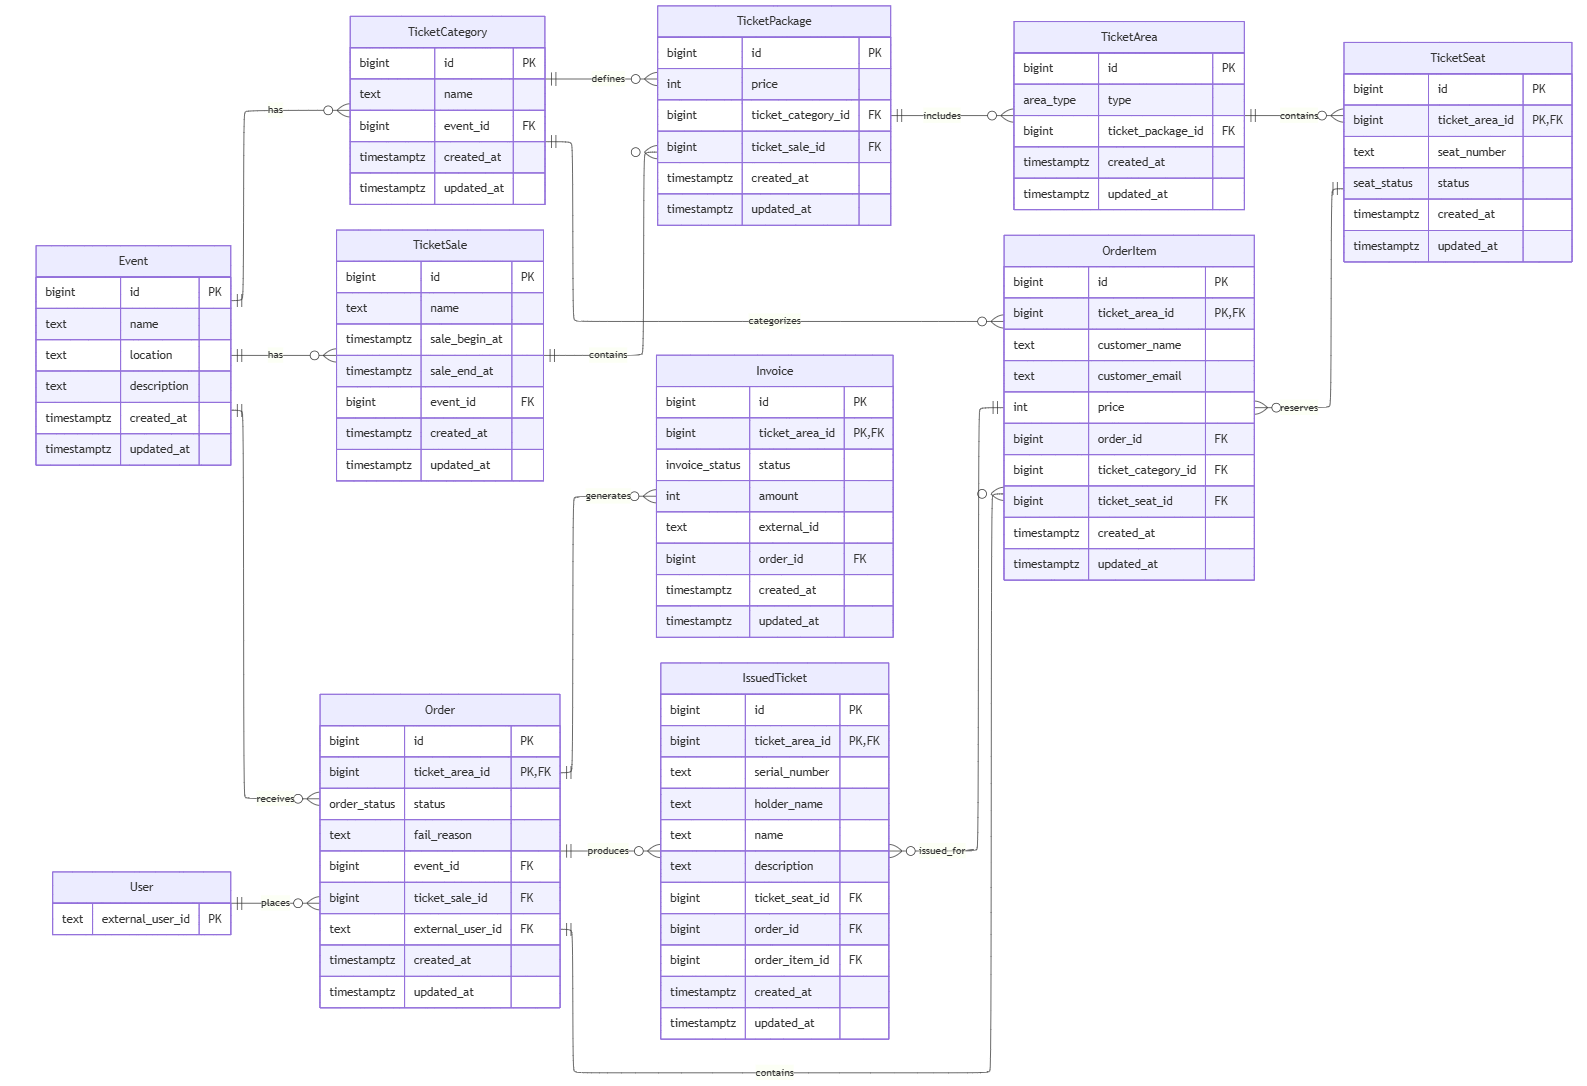
\includegraphics[width=1\textwidth]{resources/chapter-3/erd.png}
    \caption{ERD Sistem Tiket}
    \label{fig:ticket-system-erd-proposal}
\end{figure}

Berikut adalah pembagian entitas berdasarkan layanan:

\begingroup
\begin{longtable}{|p{0.3\textwidth}|p{0.6\textwidth}|}
    \caption{Pembagian Entitas Berdasarkan Layanan}                                                                                                    \\
    \hline
    \textbf{Layanan} & \textbf{Entitas}                                                                                                                \\
    \hline
    \endfirsthead

    \multicolumn{2}{|l|}{\tablename\ \thetable\ -- \textit{Lanjutan dari halaman sebelumnya}}                                                          \\
    \hline
    \textbf{Layanan} & \textbf{Entitas}                                                                                                                \\
    \hline
    \endhead

    \hline
    \multicolumn{2}{|r|}{\textit{Dilanjutkan ke halaman berikutnya}}                                                                                   \\
    \endfoot

    \hline
    \endlastfoot

    \hline
    Tiket            & Events, TicketCategory, Areas, Seats, TicketSale, \linebreak TicketPackage, Orders, OrderItem, IssuedTicket, \linebreak Invoice \\
    \hline
    \hline
    Pengguna         & Users                                                                                                                           \\
    \hline
    \hline
    Pembayaran       & Invoice                                                                                                                         \\
    \hline
\end{longtable}
\endgroup

Entitas yang berkaitan dengan acara dan tiket dibagi menjadi dua: entitas yang berkaitan dengan inventori tiket dan penjualan tiket. Entitas yang berkaitan dengan inventori meliputi TicketCategory, Areas, dan Seats. Sebuah acara bisa memiliki banyak kategori tiket, seperti tiket kategori reguler, gold, platinum. Setiap kategori tiket bisa meliputi banyak area, seperti tribun timur dan barat. Setiap area terdiri atas banyak Seat dengan status ketersediaan, yaitu tersedia, \textit{on hold}, dan terjual.

Selain itu, terdapat entitas yang berkaitan dengan penjualan tiket, yaitu TicketSale, TicketPackage. dan IssuedTicket. Entitas TicketSale menunjukkan penjualan tiket yang dilaksanakan pada batas waktu tertentu. Hal ini untuk mengakomodasi penjualan tiket untuk suatu acara yang dilakukan beberapa kali, seperti penjualan tiket \textit{early bird} dan penjualan tiket untuk umum. Setiap TicketSale memiliki banyak TicketPackage yang menandakan kategori tiket yang dijual. Entitas ini terhubung dengan entitas TicketCategory dan memiliki atribut harga serta jumlah maksimal tiket yang akan dijual. Setiap Seat menunjukkan Seat (fisik) pada hari tertentu. Tiket Seat yang sama pada hari yang berbeda akan memiliki ID yang berbeda. IssuedTicket merupakan tiket yang telah berhasil terjual dan memiliki informasi pemilik tiket dan nomor seri tiket. Entitas ini berelasi dengan Seat. Untuk menangani penjualan tiket tanpa \textit{seat}, sistem membuat \textit{virtual seat} yang akan di-\textit{assign} secara otomatis saat pembelian.

Entitas yang berkaitan dengan pembelian tiket terdiri atas entitas Users, Orders, OrderItem, dan Invoice. Terdapat dua entitas Invoice, yaitu Invoice yang disimpan dari sisi sistem tiket (sistem internal) dan Invoice yang disimpan dari sisi sistem pembayaran (sistem eksternal). Setiap pengguna bisa memesan lebih dari satu kali. Setiap pesanan terdiri atas banyak OrderItem. Entitas ini menyimpan informasi pemesan, harga saat pembayaran, dan memiliki relasi dengan TicketPackage dan Seats. Saat pembayaran berhasil, IssuedTicket akan dibuat berdasarkan informasi OrderItem. Selain itu, terdapat entitas Invoice yang menyimpan informasi yang berkaitan dengan tagihan pembayaran.